\documentclass[12pt,letterpaper]{report}
\usepackage[margin=1in]{geometry}
\usepackage{graphicx}
\usepackage{amsmath}
\usepackage[font=small,labelfont=bf]{caption}
\usepackage[justification=centering]{caption}
\usepackage{tikz}
\usepackage{circuitikz}
\usepackage{siunitx}
\usepackage{float}
\newlength \figwidth
\setlength \figwidth {0.75\linewidth}

\begin{document}

\title{E153 Laboratory Assignment \#9}
\author{Courtney Keeler and Stephen Pinto\\
Harvey Mudd College}
\date{December 18, 2013}
\maketitle

\section*{List of Materials}
\begin{itemize}
	\item Tektronix 2212 Oscilloscope
	\item Pomona 4550B (10X probe)
	\item Elenco LCM-1950 Multimeter
	\item Spectrum Analyzer
	\item 411 Comparator
	\item Standard resistors
	\item Standard capacitors
	\item \#344 lamp
\end{itemize}

\section*{Purpose}
The purpose of this lab is to explore the characteristics of a Wien-Bridge oscillator using a \#344 lamp as the negative feedback variable resistance.

\section*{Input Resistance Determination}

By varying the resistance on the decade resistance box, the best input resistance was found to be 101 $\Omega$. Figure \ref{fig:before} shows the Wien-Bridge oscillator with the original 560 $\Omega$ input resistance. Notice that the oscillation amplitude has increased to the point that it hit the opamp rails and created a square wave (really, this is a very distorted sine wave). Figure \ref{fig:after} shows the output of the oscillator circuit with a decreased load. It is very hard to eliminate the distortion completely, however the final resistor value chosen minimized it the most without comprimising the sine wave output.

\begin{figure}[H]
\centering
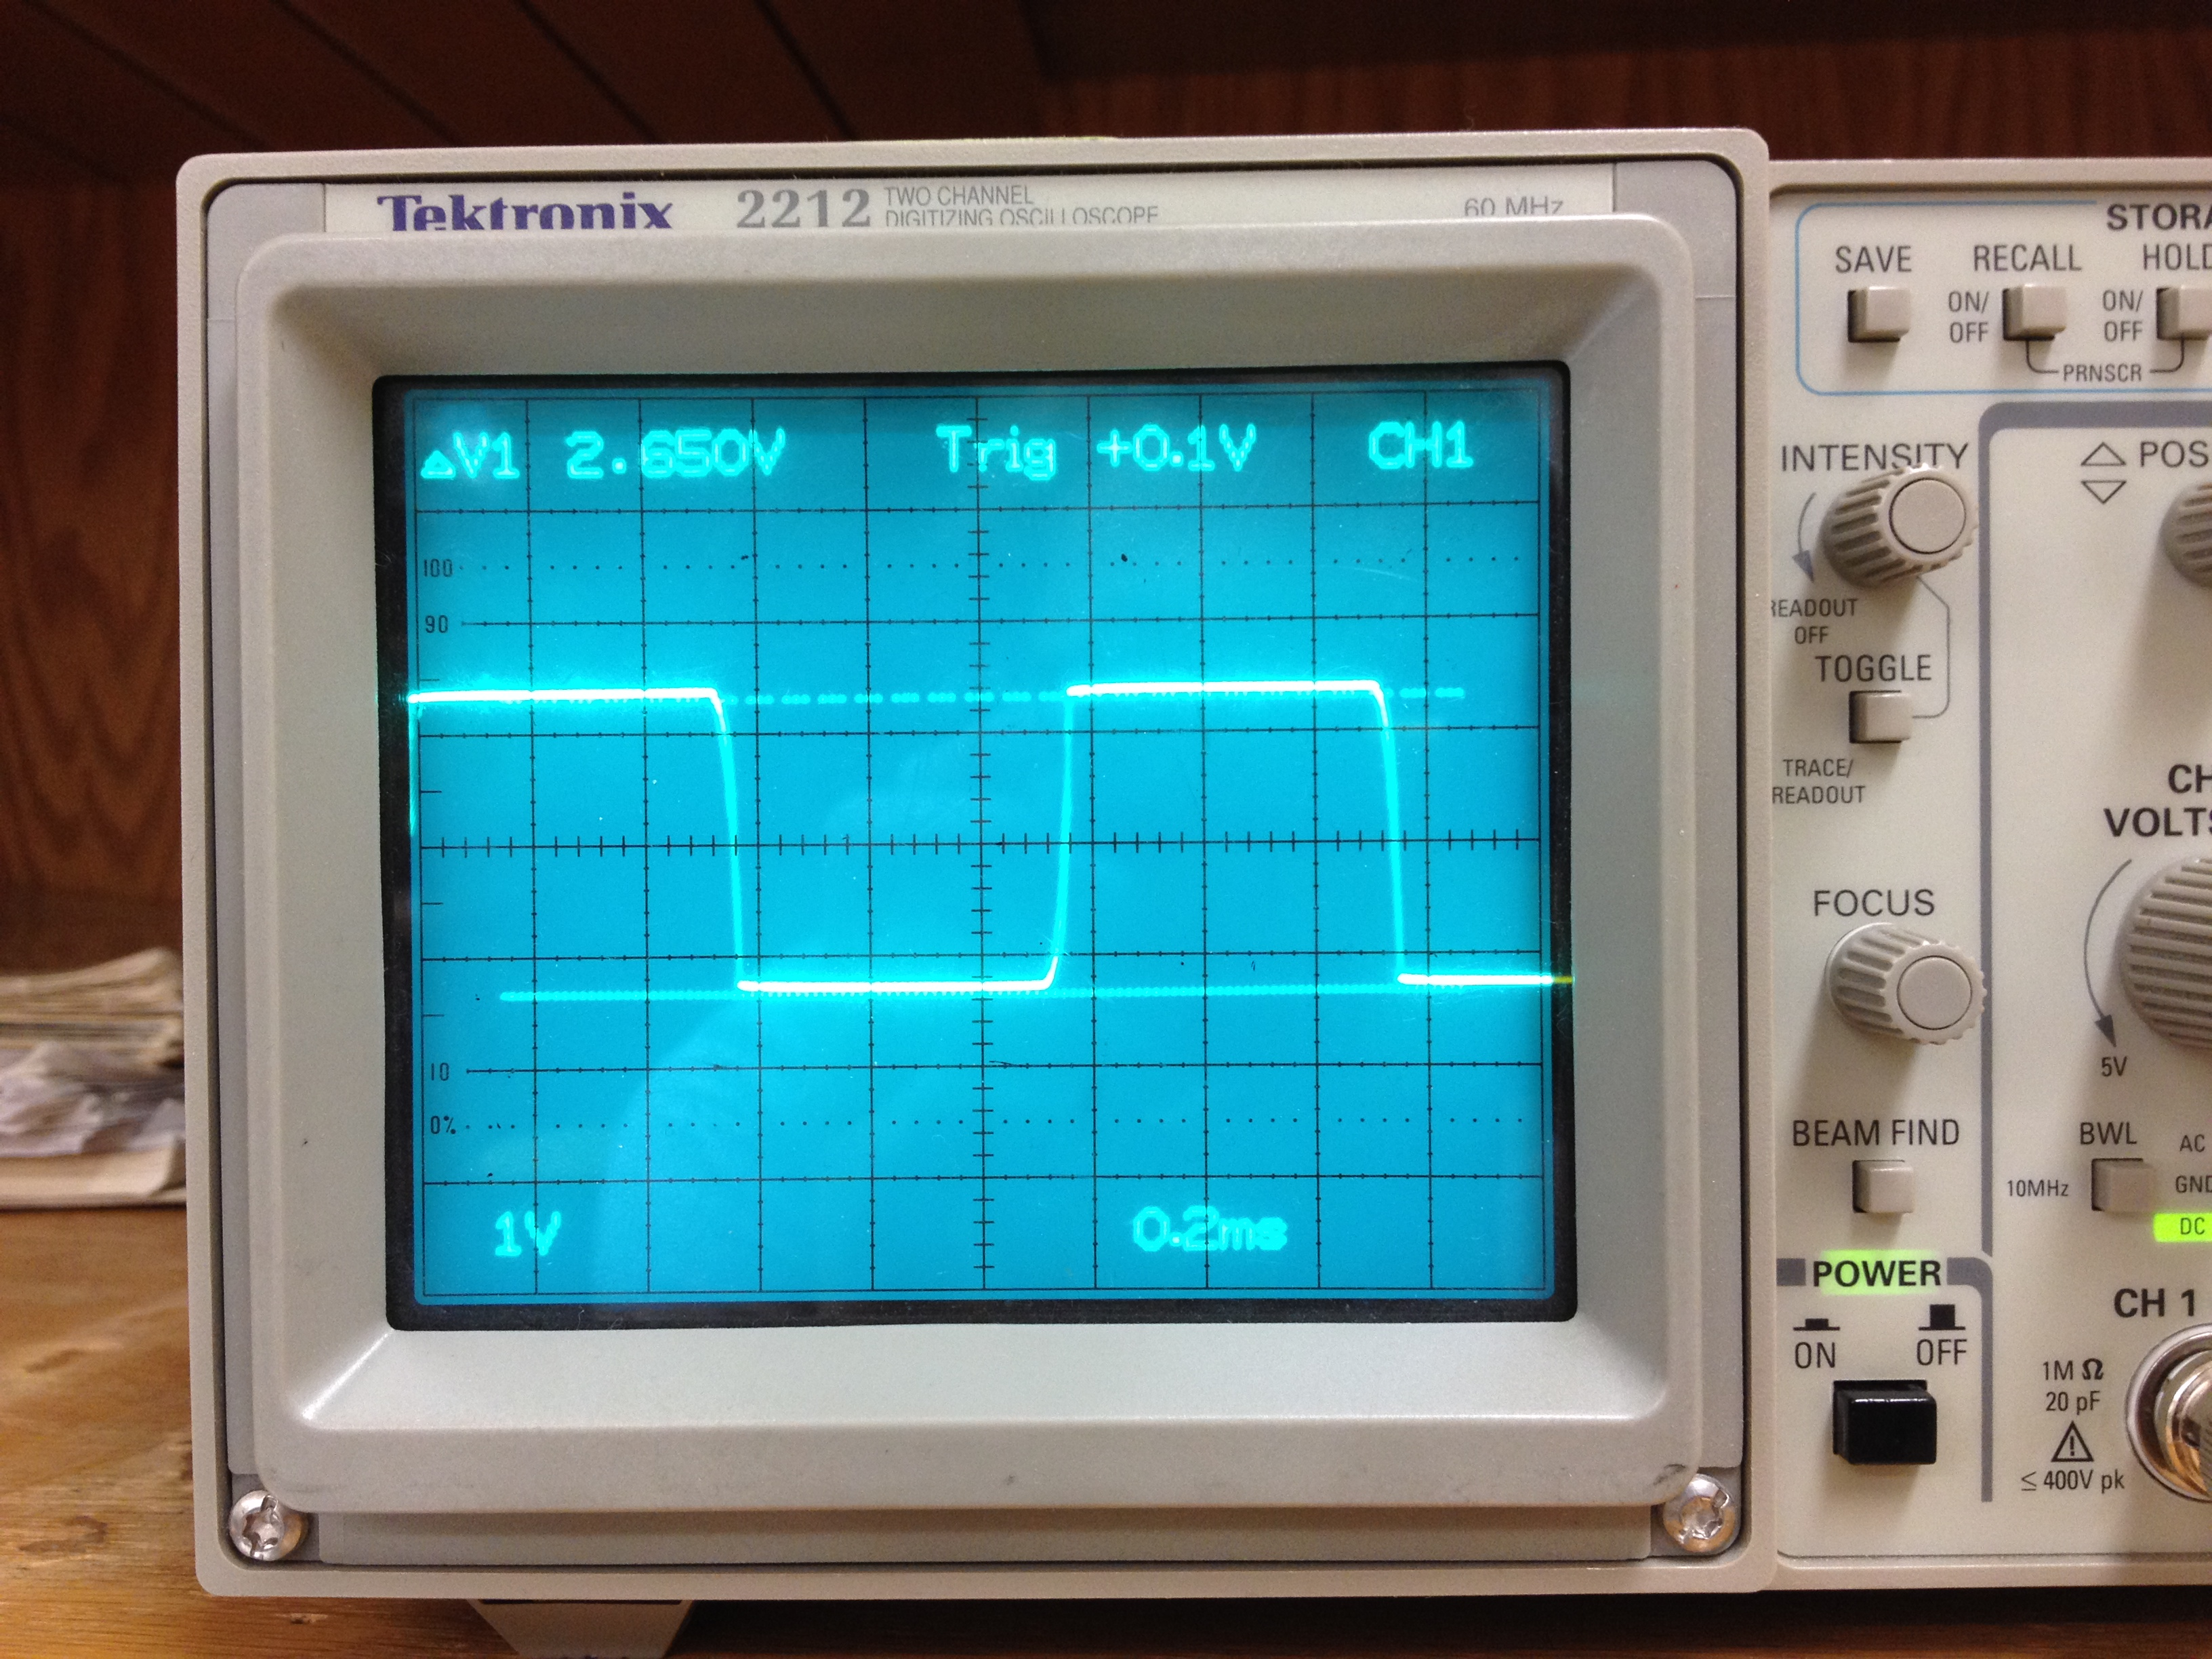
\includegraphics[width=\figwidth, keepaspectratio=true]{lab9_images/before.jpg}
\caption{Output of the Lab 9 Wien-Bridge oscillator with negative feedback resistance of 560 $\Omega$.}
\label{fig:before}
\end{figure}

\begin{figure}[H]
\centering
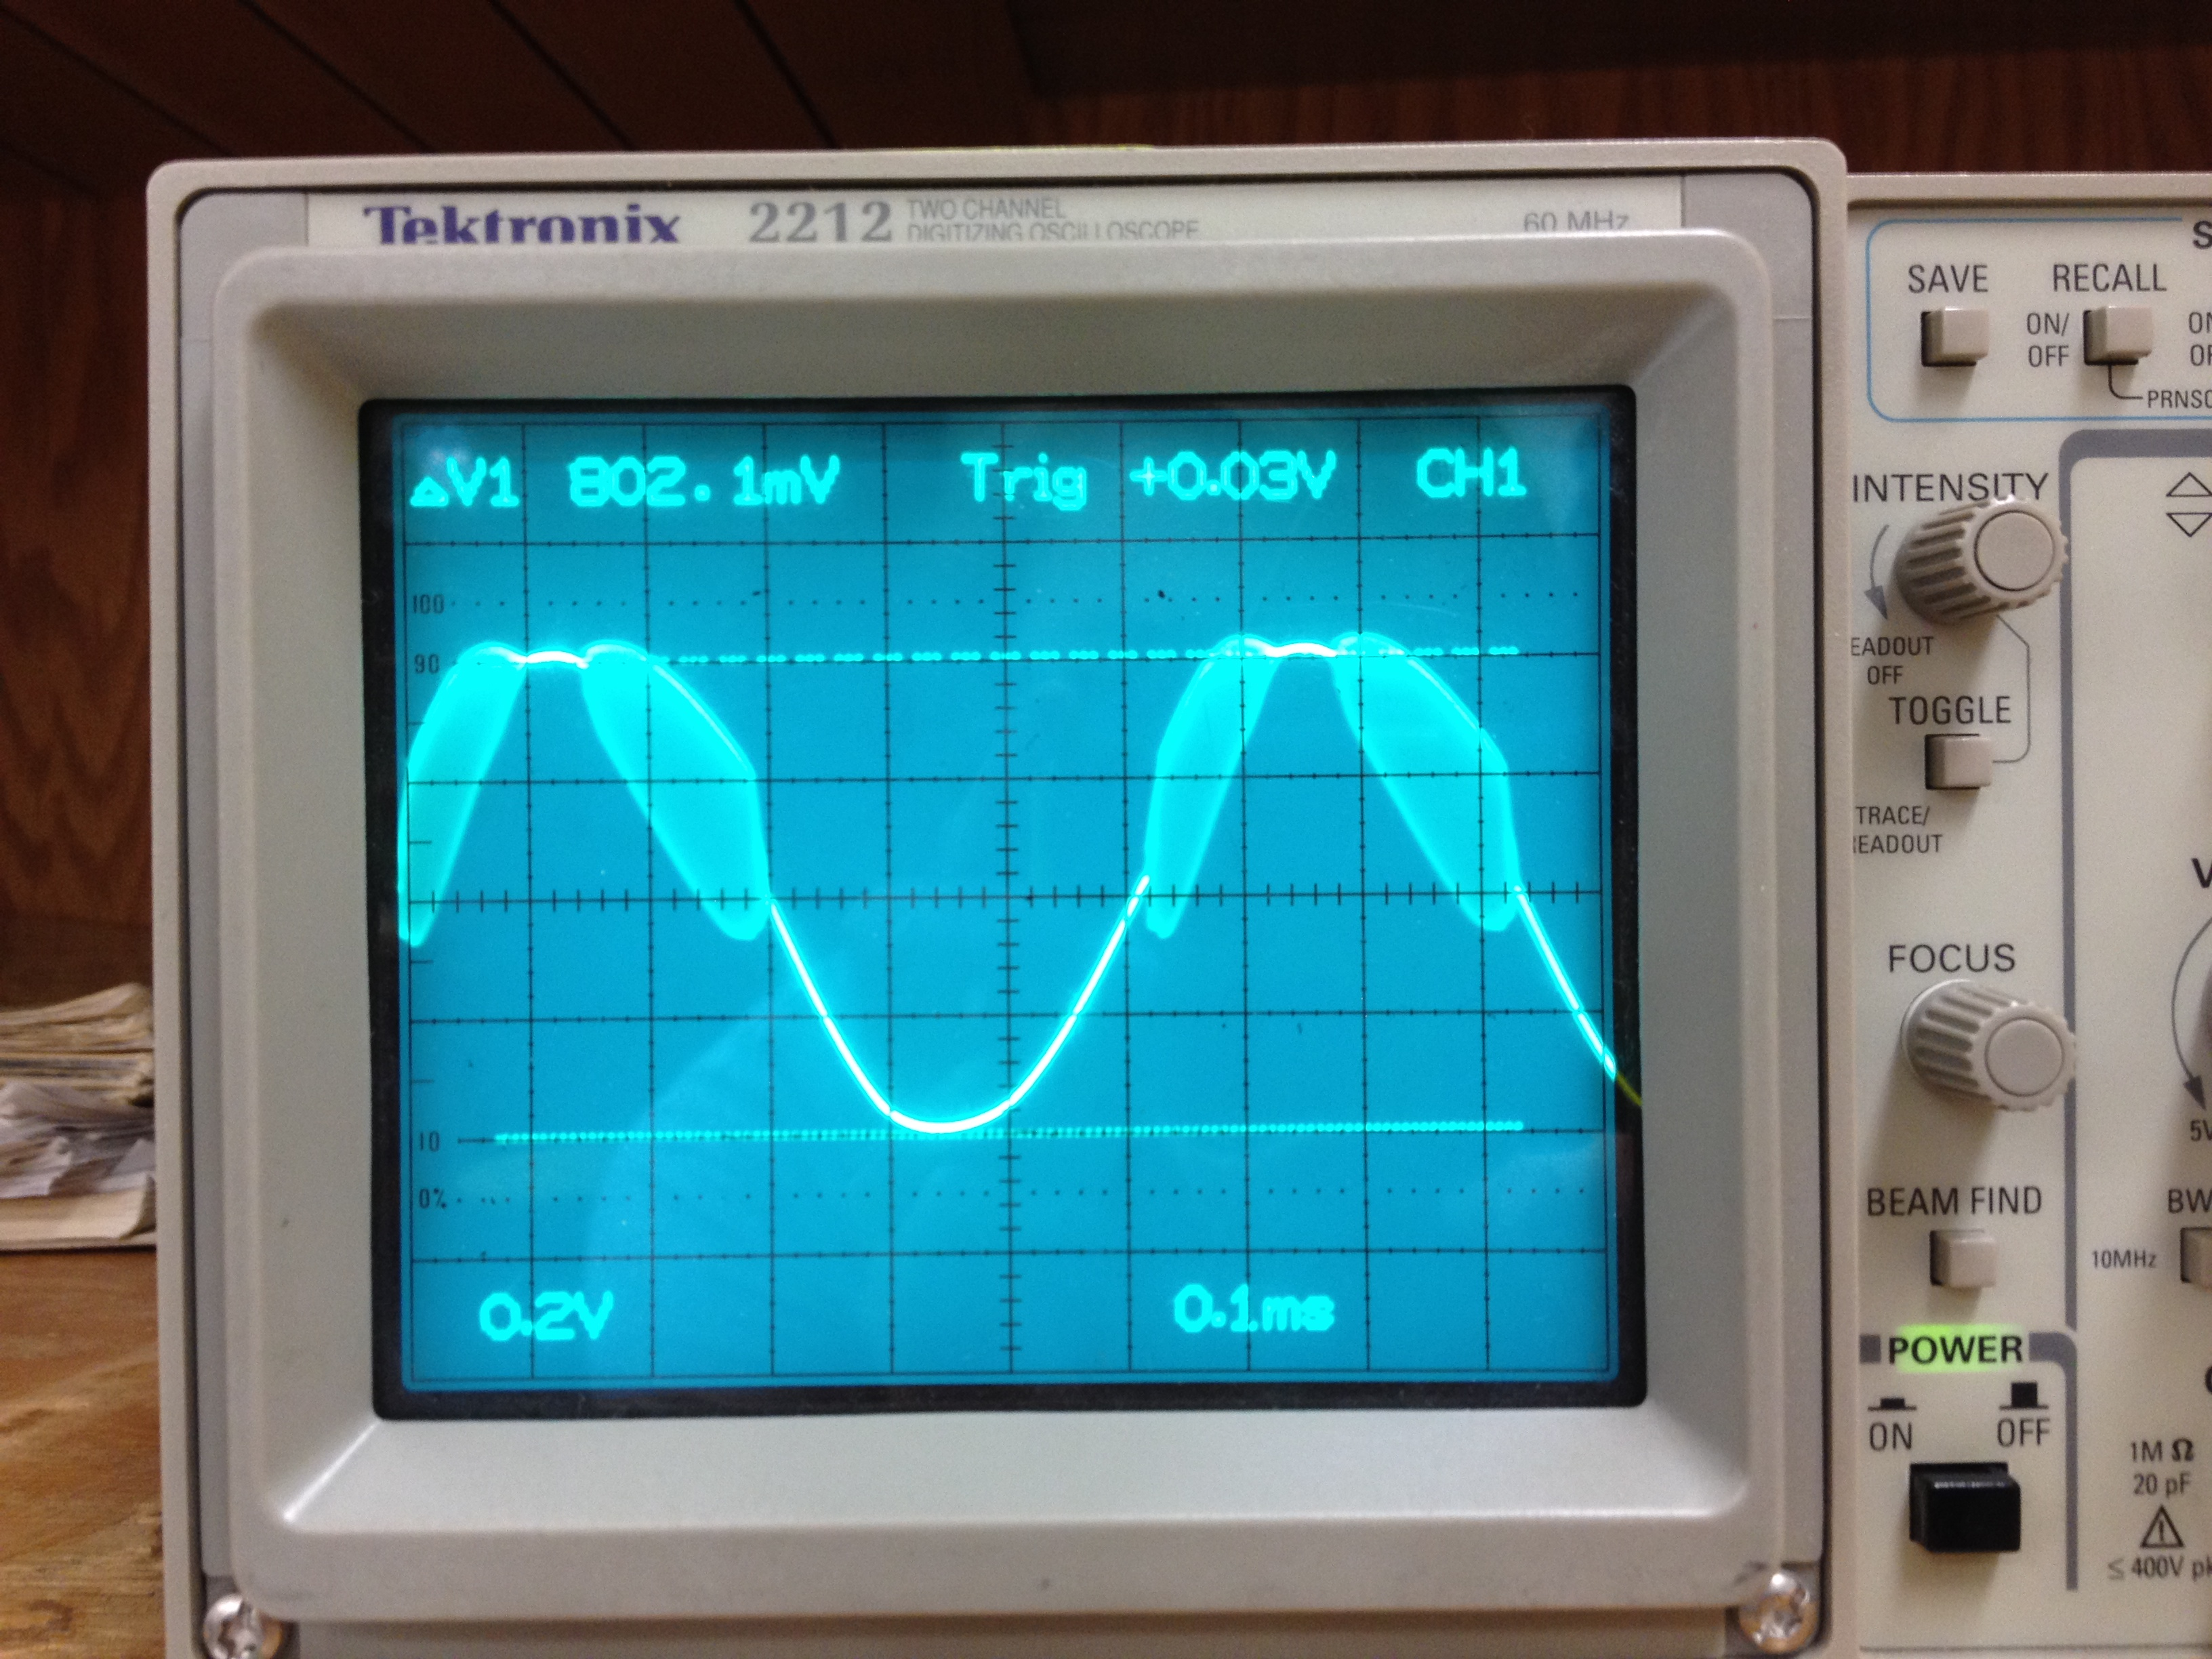
\includegraphics[width=\figwidth, keepaspectratio=true]{lab9_images/after.jpg}
\caption{Output of the Lab 9 Wien-Bridge oscillator with negative feedback resistance of 101 $\Omega$.}
\label{fig:after}
\end{figure}

\section*{Comparison with Function Generator}

The next step is to examine the frequency components using the spectrum analyzer. Figure \ref{fig:circuit_spec} shows the spectral analysis of the Wien-Bridge oscillator circuit. Notice the highest frequency component of the signal is at 1.5 kHz, which corresponds with the expected oscillator output frequency. However, there are also small frequency components that occur at higher frequencies. These are due to the fact that a square wave, which is what the distorted Wien-Bridge output becomes for high negative feedback resistances, is a combination of many different frequency sine waves. The dominant frequency component of a square wave will be the natural frequency, but at 1/3, 1/5, 1/7, etc. of the natural frequency, there will also be small contributions. Since the Wien-Bridge oscillator output is not a perfect sine wave, we see these small contributions at higher frequencies.

\begin{figure}[H]
\centering
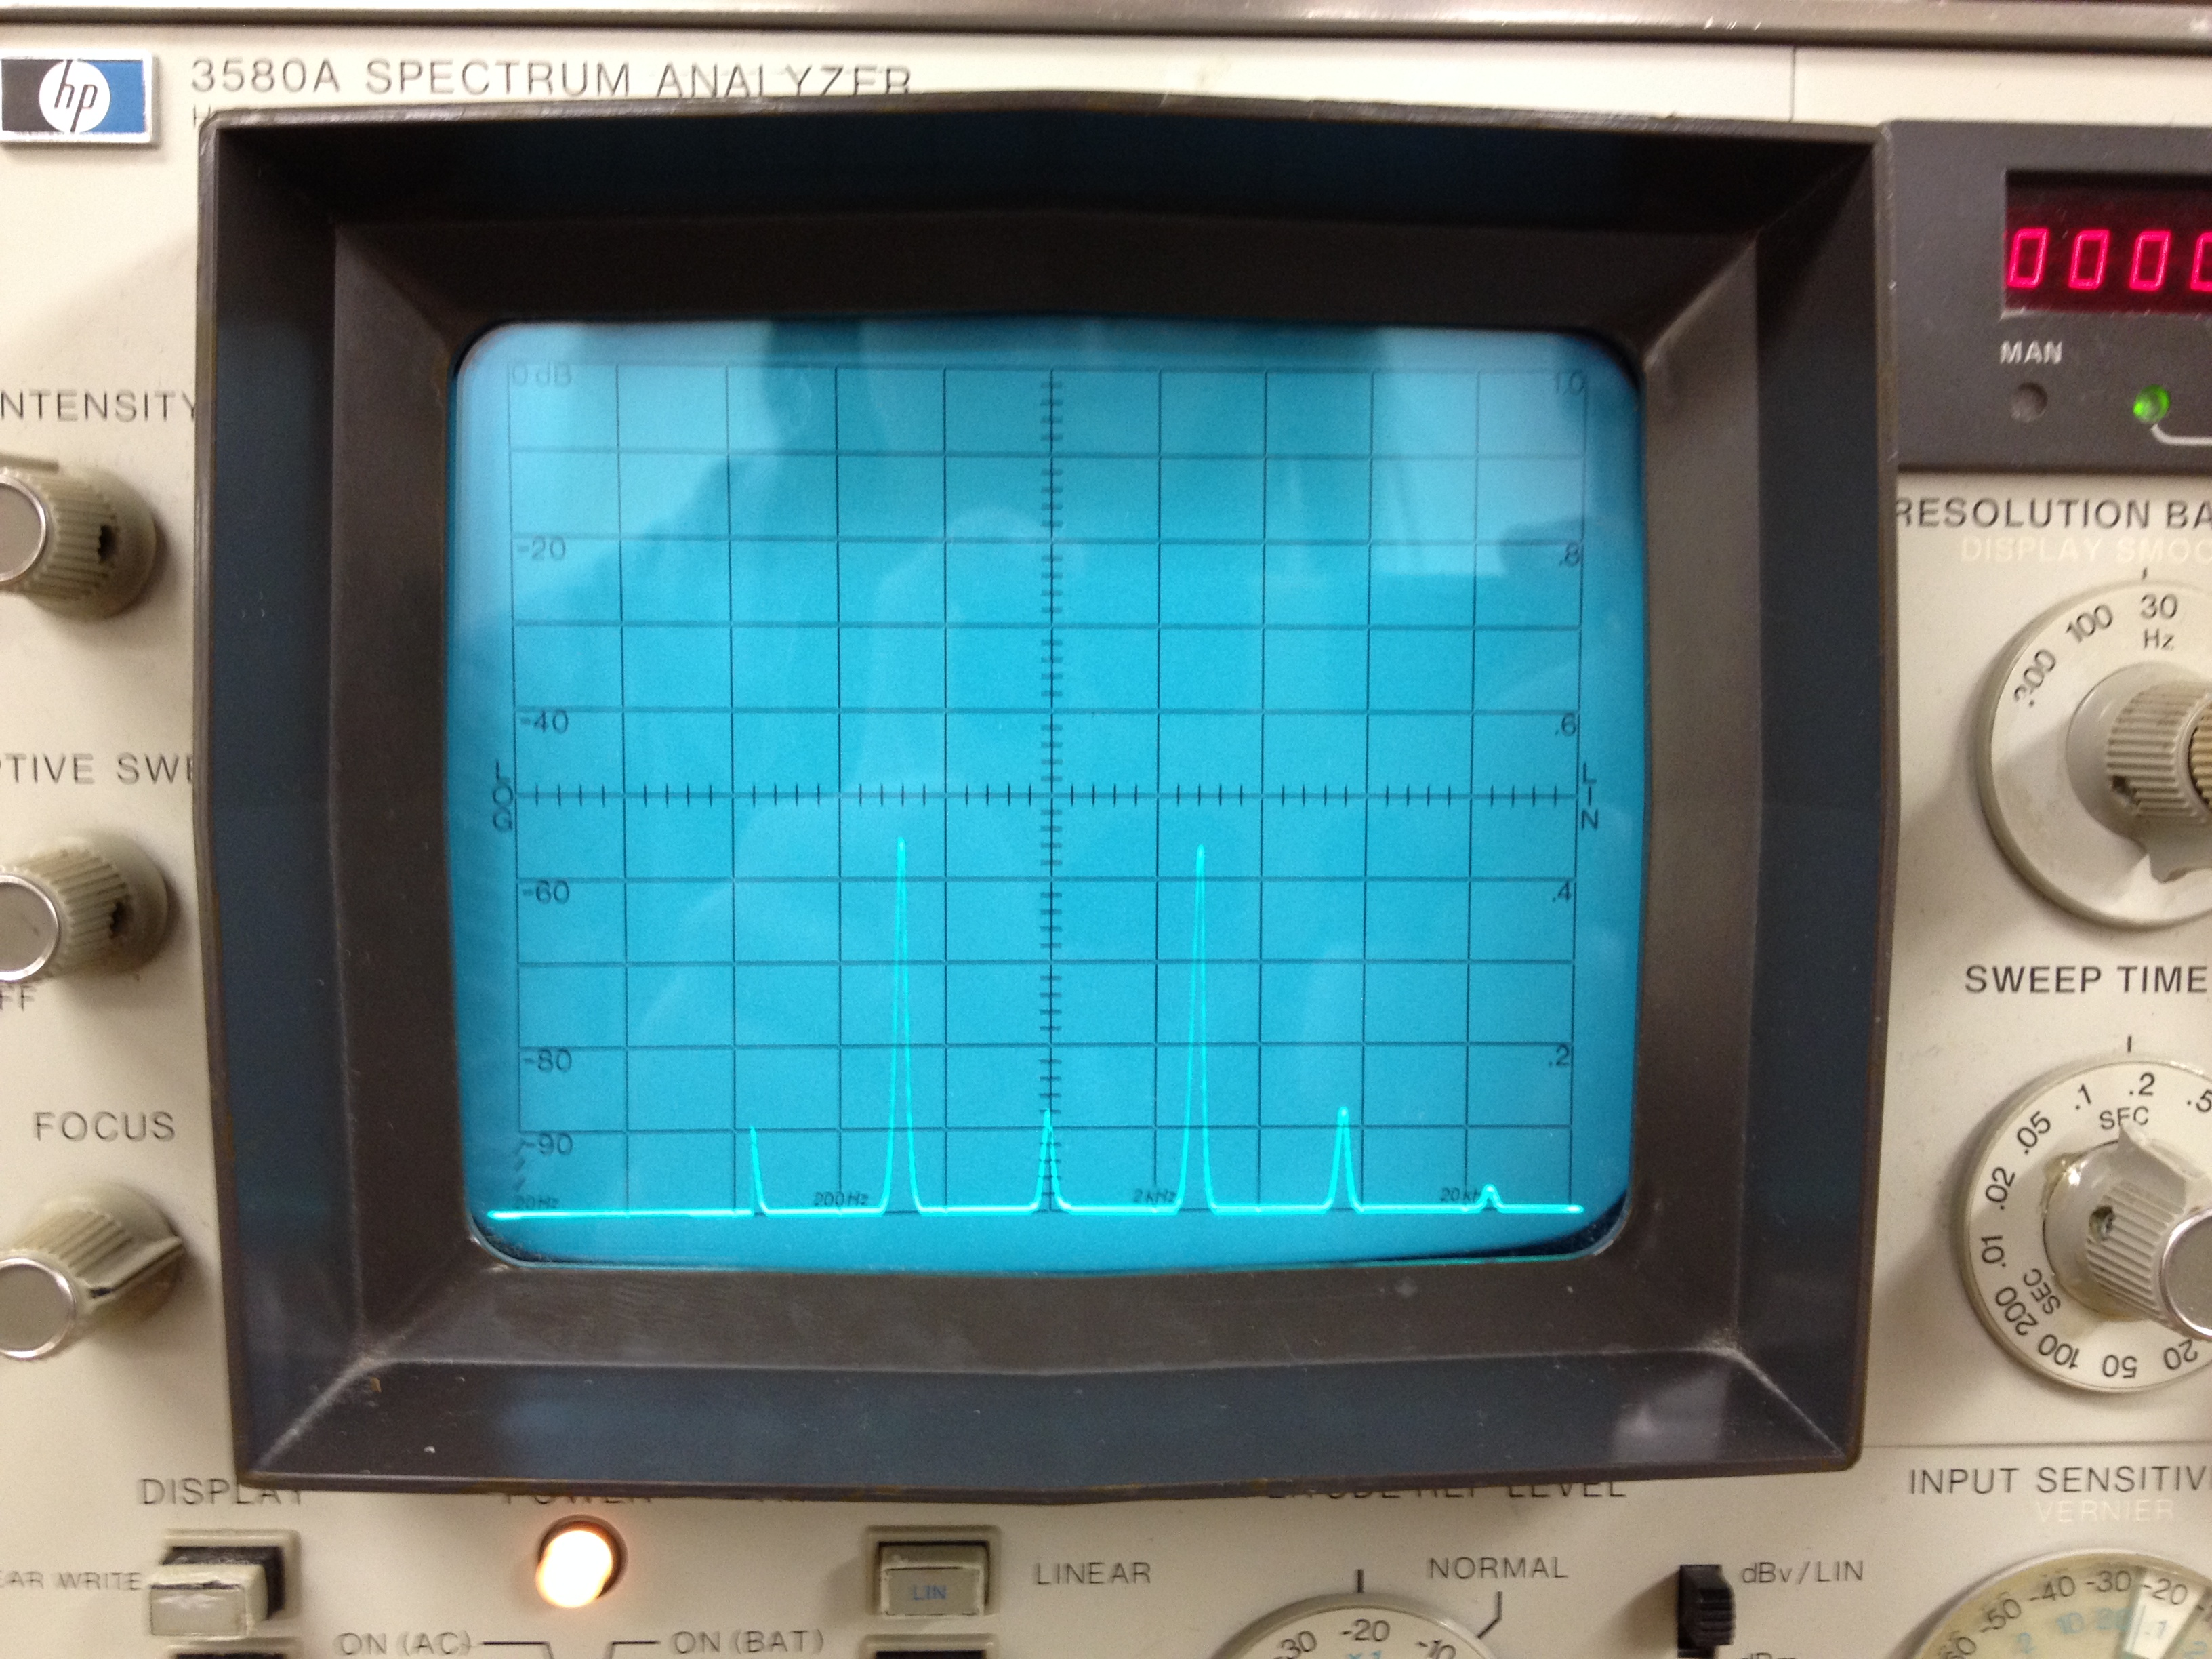
\includegraphics[width=\figwidth, keepaspectratio=true]{lab9_images/circuit_spec.jpg}
\caption{Spectral analysis (double-sided spectrum, x0.1 amplification) of the Wien-Bridge oscillator circuit output.}
\label{fig:circuit_spec}
\end{figure}

\begin{figure}[H]
\centering
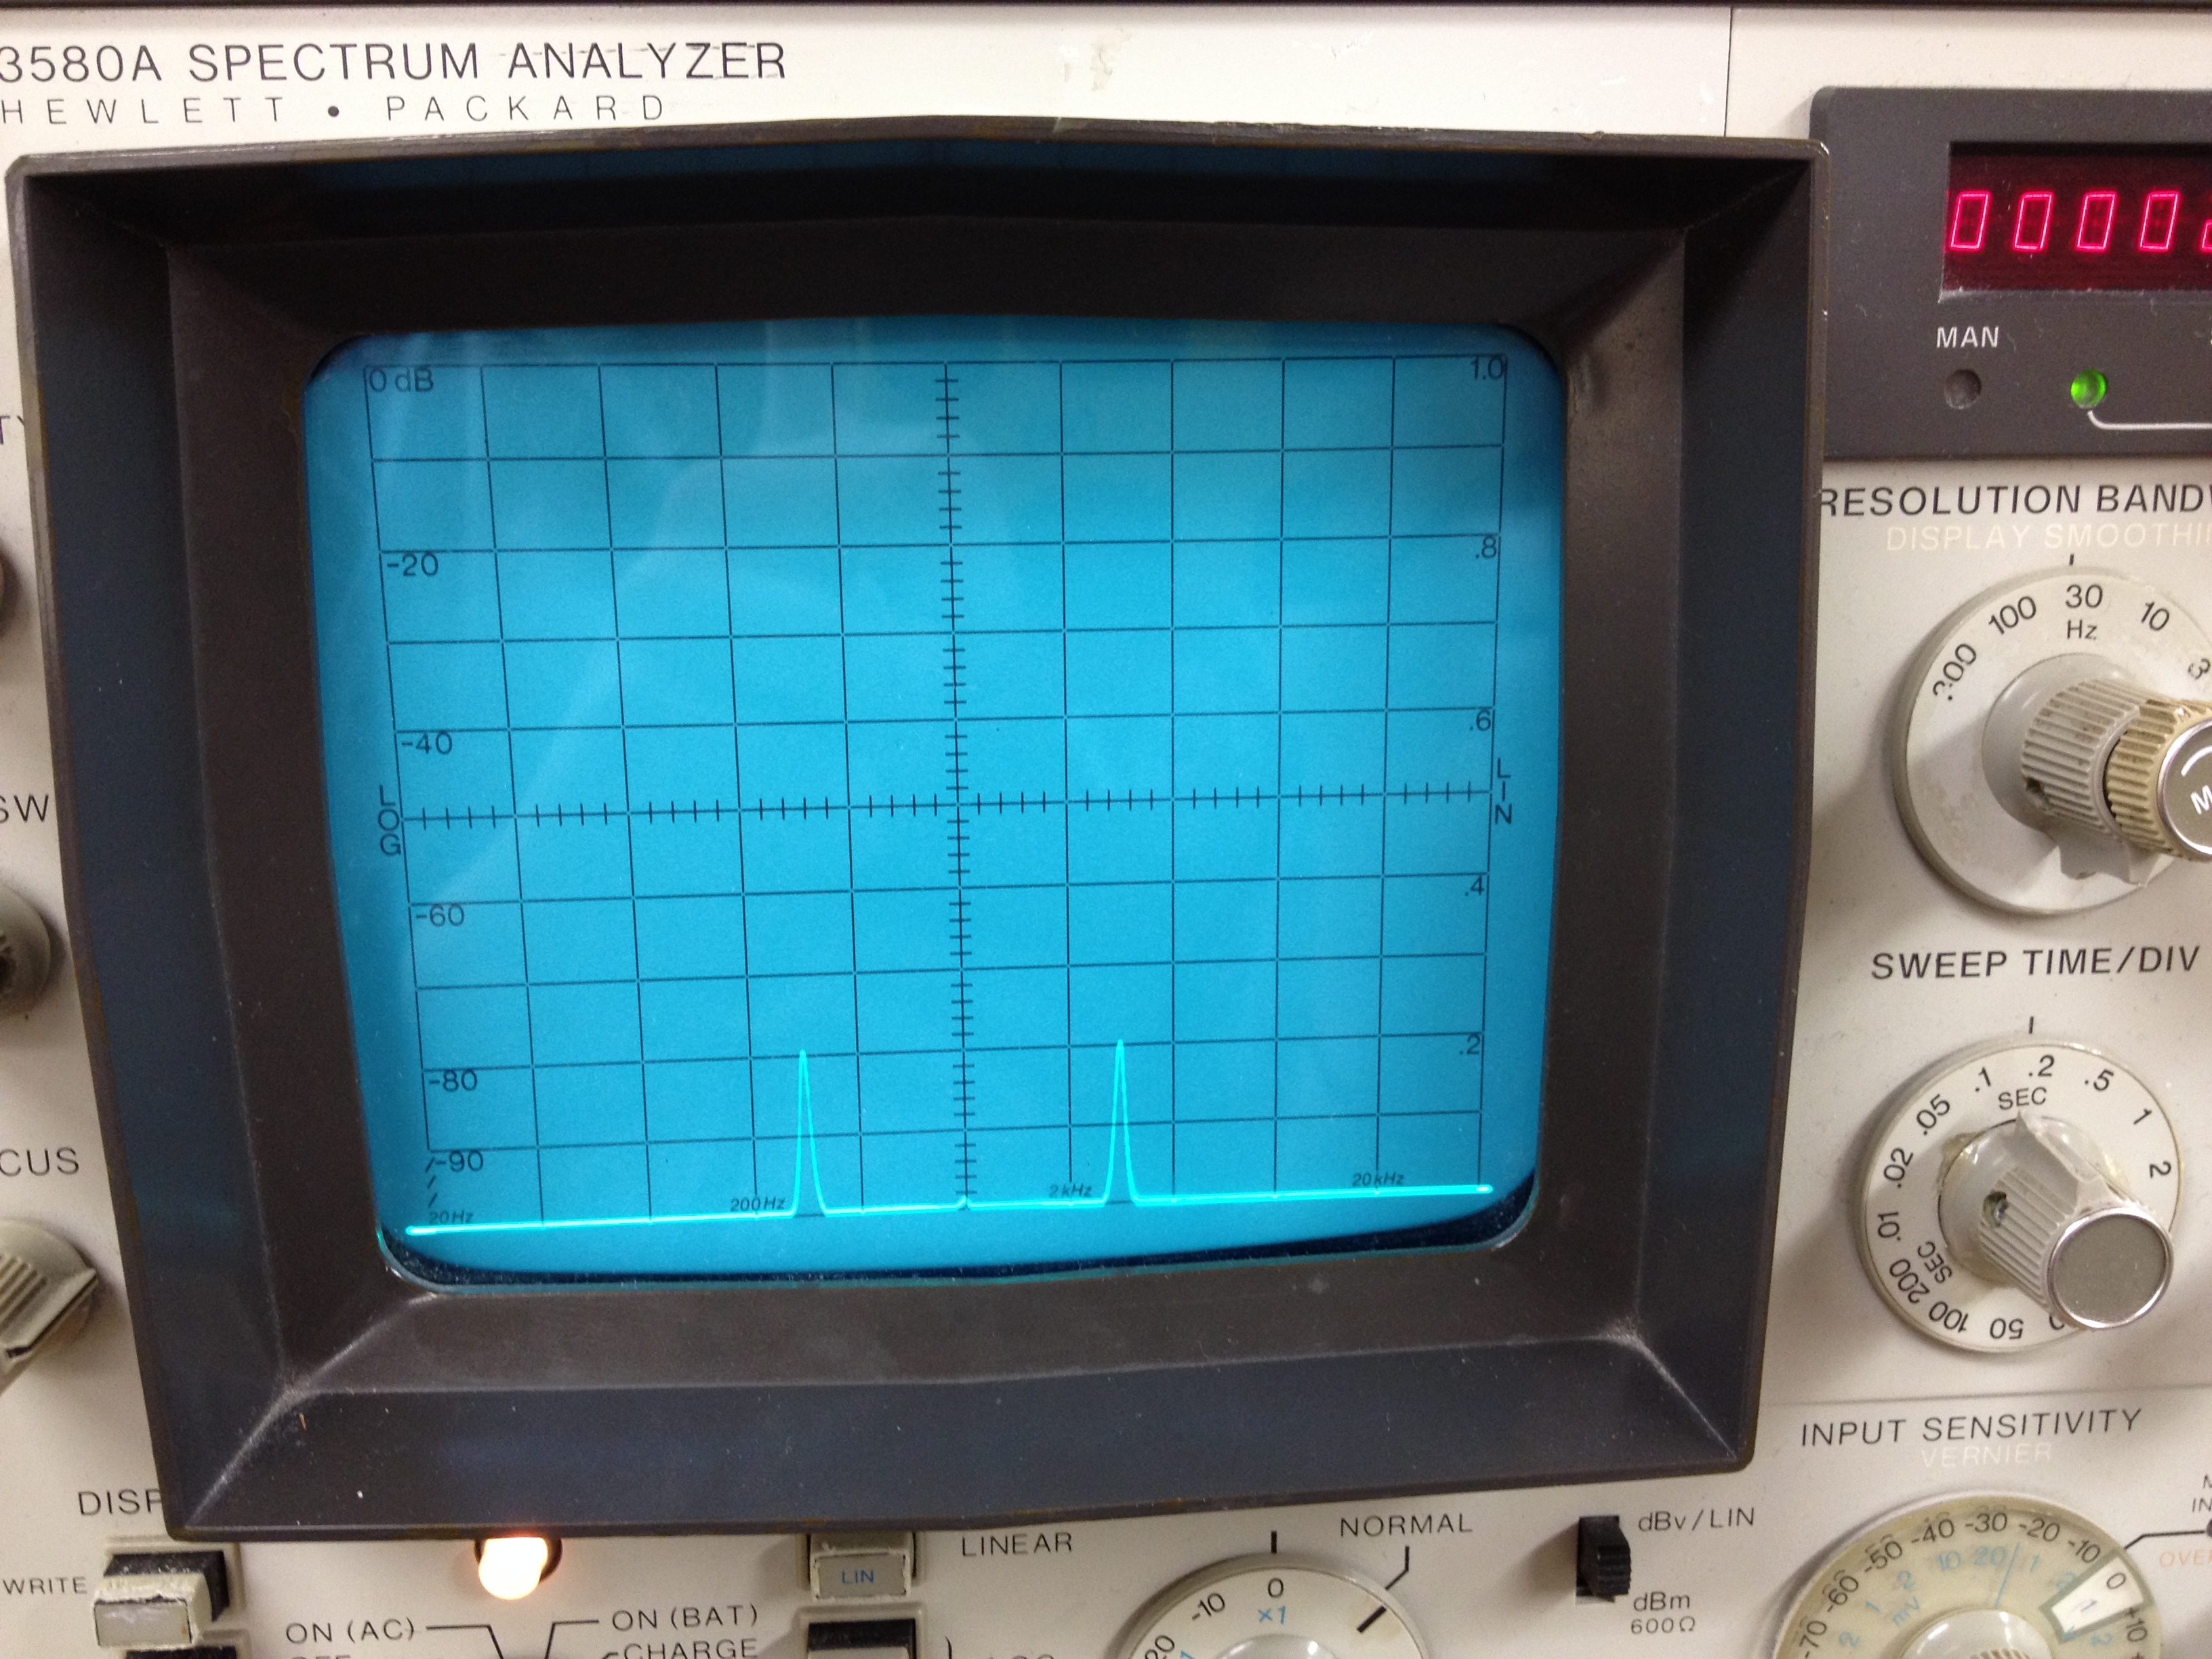
\includegraphics[width=\figwidth, keepaspectratio=true]{lab9_images/gen_spec.jpg}
\caption{Spectral analysis (double-sided spectrum, x0 amplification) of a 1.5 kHz frequency sine wave generated by a function generator.}
\label{fig:gen_spec}
\end{figure}

Figure \ref{fig:gen_spec} shows the spectral analysis of a function generator 1.5 kHz sine wave. Here, since the sine wave is pure, there is only one frequency component occurring at 1.5 kHz on the spectral plot. 

\section*{Analysis and Observations}

As the previous section showed, the function generator output is a much cleaner signal than the Wien-Bridge oscillator. However, depending on the application, the difference might be tolerable. 
The cause of the distortion of the output sinusoid from the Wien-Bridge is the non-linear opamp. An opamp is comprised in part of transistors and diodes, both of which are non-linear elements in the lab (though we sometimes simplify their behavior to linear regions for circuit analysis).

In order to get a cleaner signal out of the Wien-Bridge oscillator, it is possible to use an even smaller negative feedback resistance value. However, there are two considerations to make. First, the negative feedback resistance cannot drop below the RC frequency-determining network, otherwise the system will not oscillate. Second, with a lower resistance value, the opamp gain decreases as well. This means the signal may need additional amplification down the line since the output will be only a small fraction of the opamp rail-to-rail voltage.

\section*{Conclusion}

In conclusion, this lab has shown the effects of the negative feedback resistance of the WIen-Bridge oscillator circuit. In the future, this knowledge can be used to choose the proper resistor value in a custom Wien-Bridge oscillator design. The purposes of the lab, which were to build the Wien-Bridge circuit and compare the behavior to a function generator, were clearly met and detailed herein.

\end{document}
